\chapter{Observing at the Marion Island Site}

\attention{You have all the right factors for site selection in the
  paragraphs below, but I'll suggest reorganizing for clarity.  Start
  by explicitly stating that there are several factors that need to be
  considered when choosing a site for PRIZM/ALBATROS, and that those
  are RF quietness, ionospheric conditions, accessibility, and ability
  to support long baselines.}

Low-frequency observations require high angular resolution to improve the experiment's sensitivity. Systematics discussed in \S\ref{s:chall} widely dominate the experiments operating at frequencies $<$\SI{200}{MHz}. RFI from the frequency modulation (FM) transmitters is a substantial contributor in the low-frequency regime; thus, FM contamination is widespread into observation bands. Observing from remote deployment sites is a solution to the FM band contamination issue. Before site selection and deployment, radio environments must match the specific instrument's requirements when assessed. Accessibility is a common challenge that arises from remote site selection. Therefore, choosing a good observing location is generally a balance between	accessibility and radio-quietness. 

Marion Island was chosen as the observing site for Probing Radio Intensity at high-Z from Marion~\citep[\prizm;][]{2019JAI.....850004P} and the Array of Long Baseline Antennas for Taking Radio Observations from the Sub-Antarctic~\citep[\albatros;][]{2020arXiv200812208C} \attention{[since you've defined PRIZM and ALBATROS as acronyms already, there's no need to redefine them here]} after evaluating the mentioned factors. Marion Island is the exceptionally radio-quiet environment for low-frequency observations, although the site is only accessible annually. The next section discusses the location in more detail.

\section{Marion Island}

Marion Island is a research base that forms part of the Prince Edward Islands shown in Figure~\ref{fig:marion}, located in the southern Indian Ocean at \ang{46;54;45}S, \ang{37;44;37}E. The South African National Antarctic Programme (SANAP) and the South African Department of Environmental Affairs (DEA) operate the research base shown in Figure~\ref{fig:base}. \attention{[I edited some of the text in the next few sentences.]} The island is $\sim$ \SI{2000}{\kilo\metre} from the nearest continental landmasses, has an area of 290~km$^2$, and the main base is positioned on the northeast side. Marion Island has a volcanic origin, and the terrain is scattered with many secondary craters and small lakes. There is abundant snow and rain, and the vegetation is mainly mosses and ferns. The lowland regions are marshy due to high precipitation. It is extremely windy and	mostly cloudy throughout the year.

\begin{figure}
	\centering
	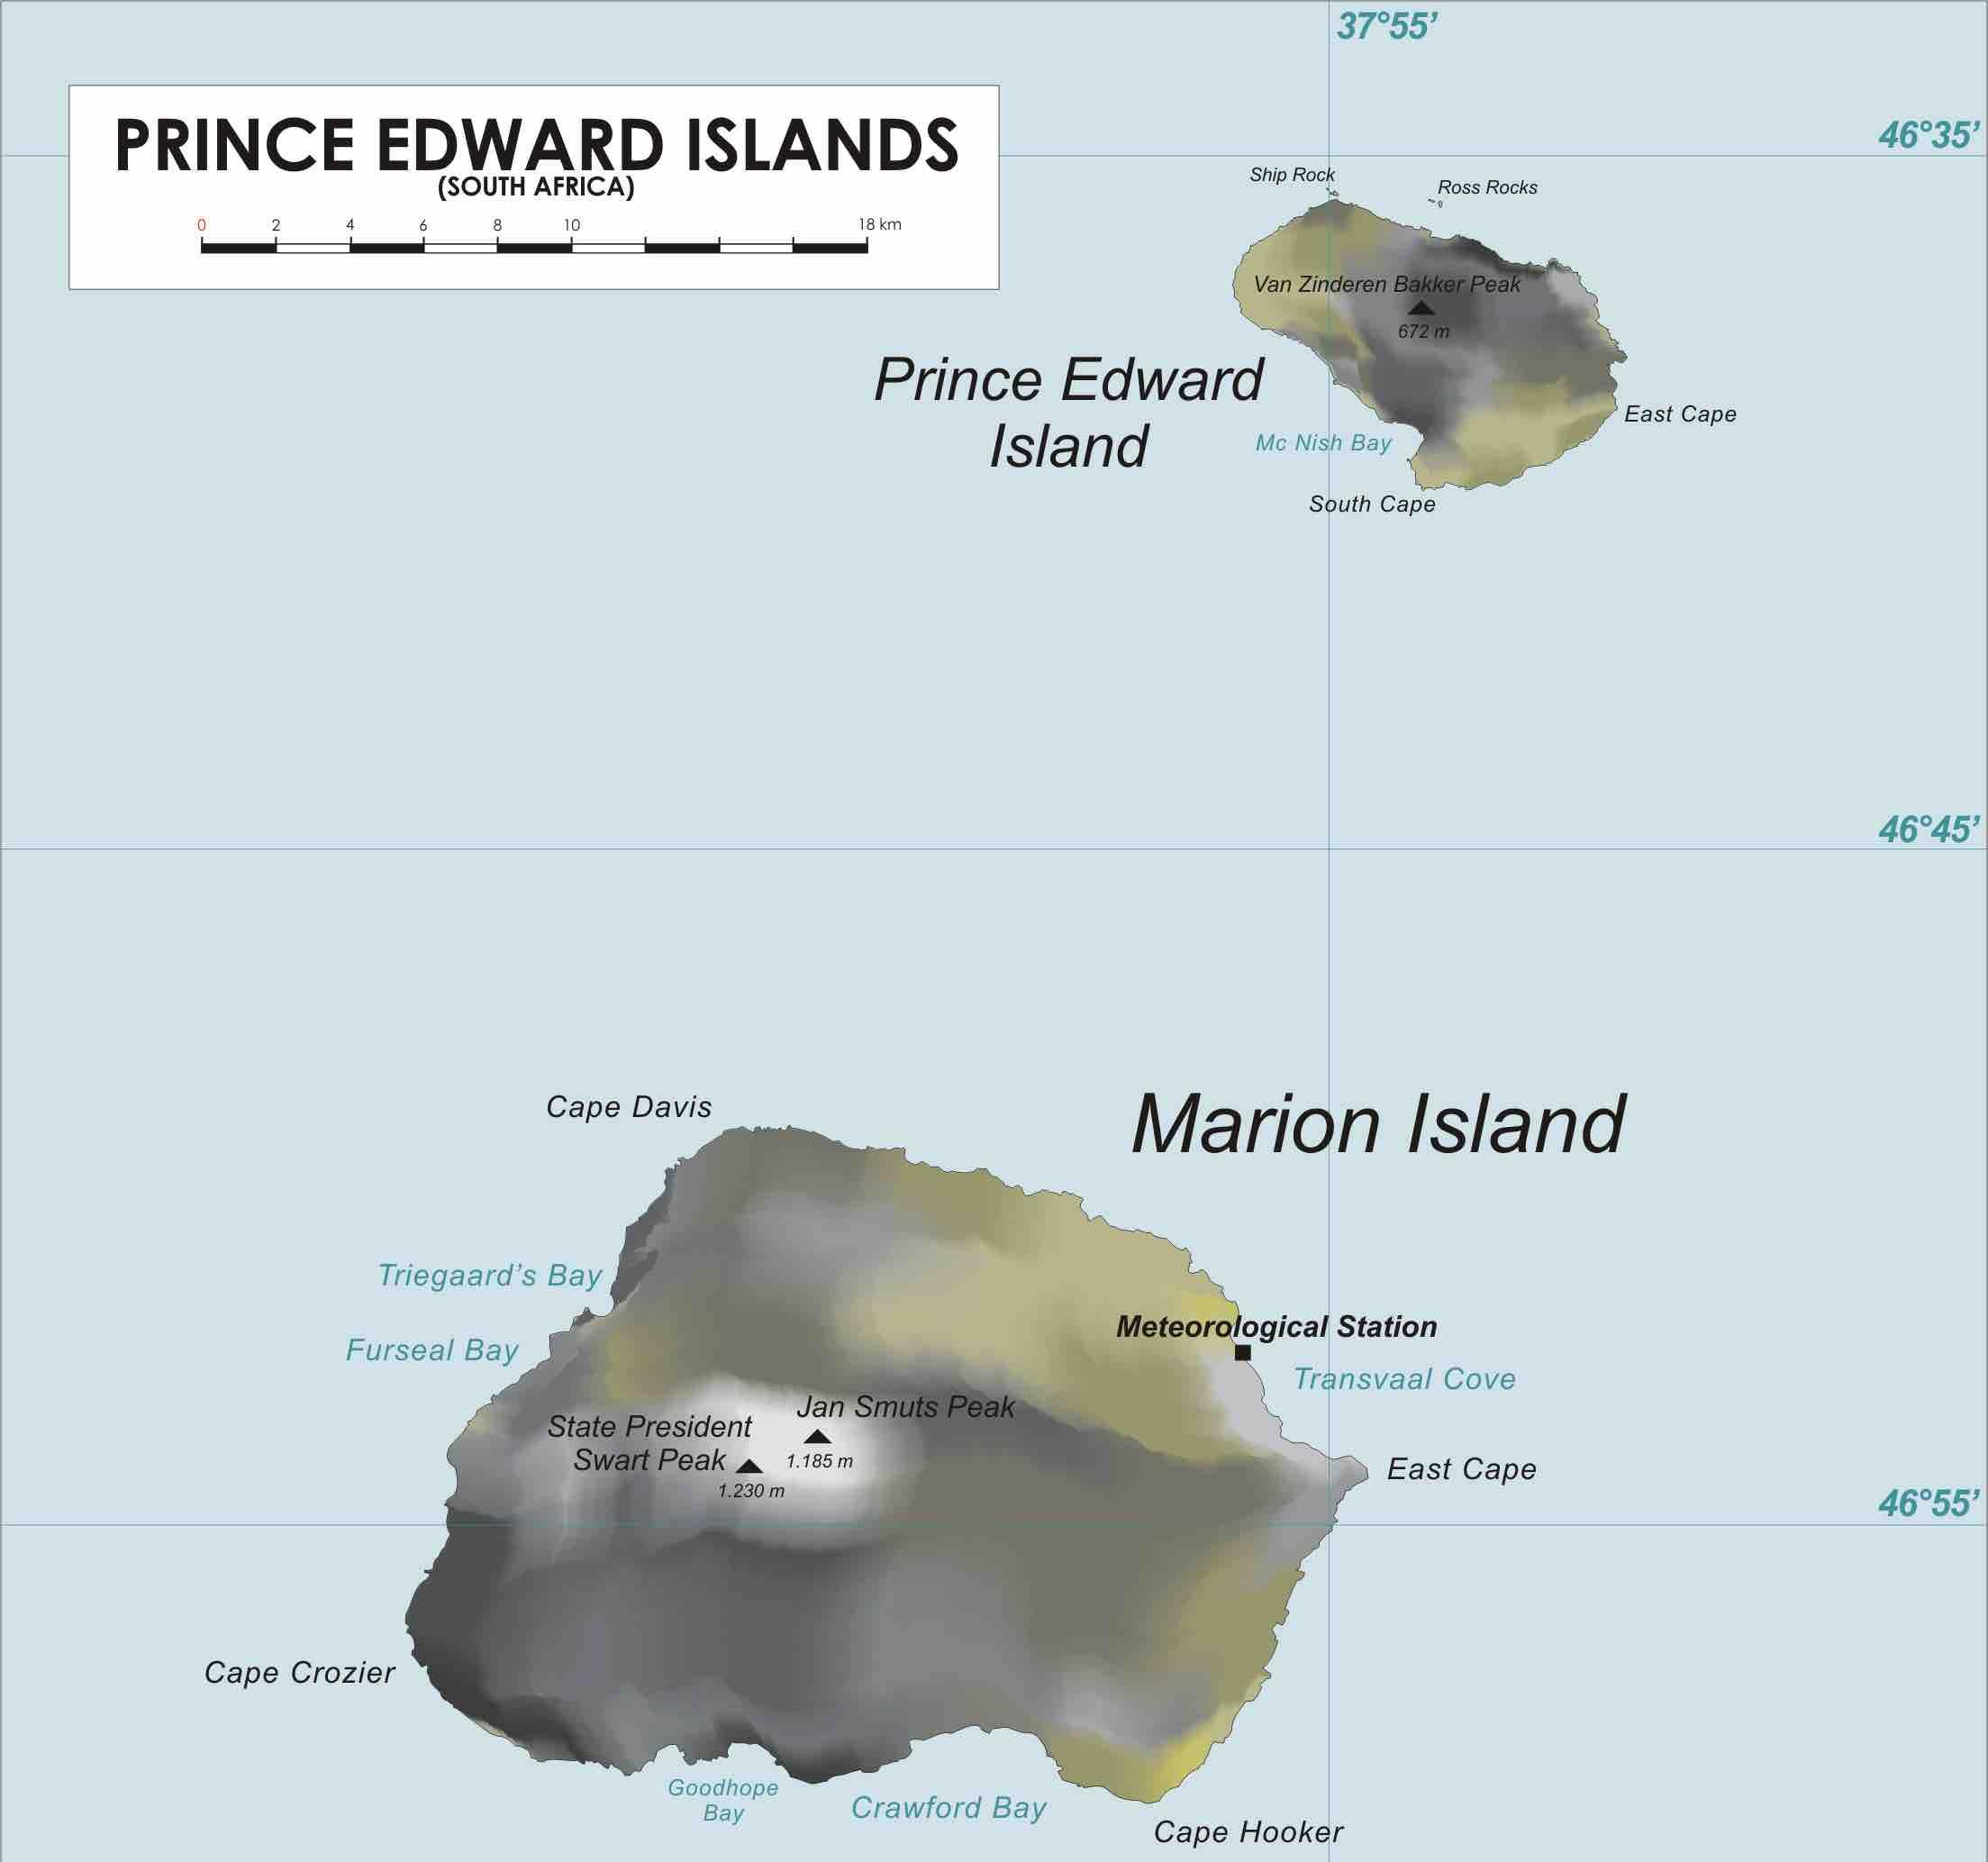
\includegraphics[width=\linewidth]{Figures/marion}
	\caption{The two islands in the Prince Edward Islands are Prince Edward Island and Marion Island, located in the sub-Antarctic Indian ocean. \attention{[I made some minor edits.  Include a source for the figure.]}}
	\label{fig:marion}
\end{figure}

\begin{figure}
	\centering
	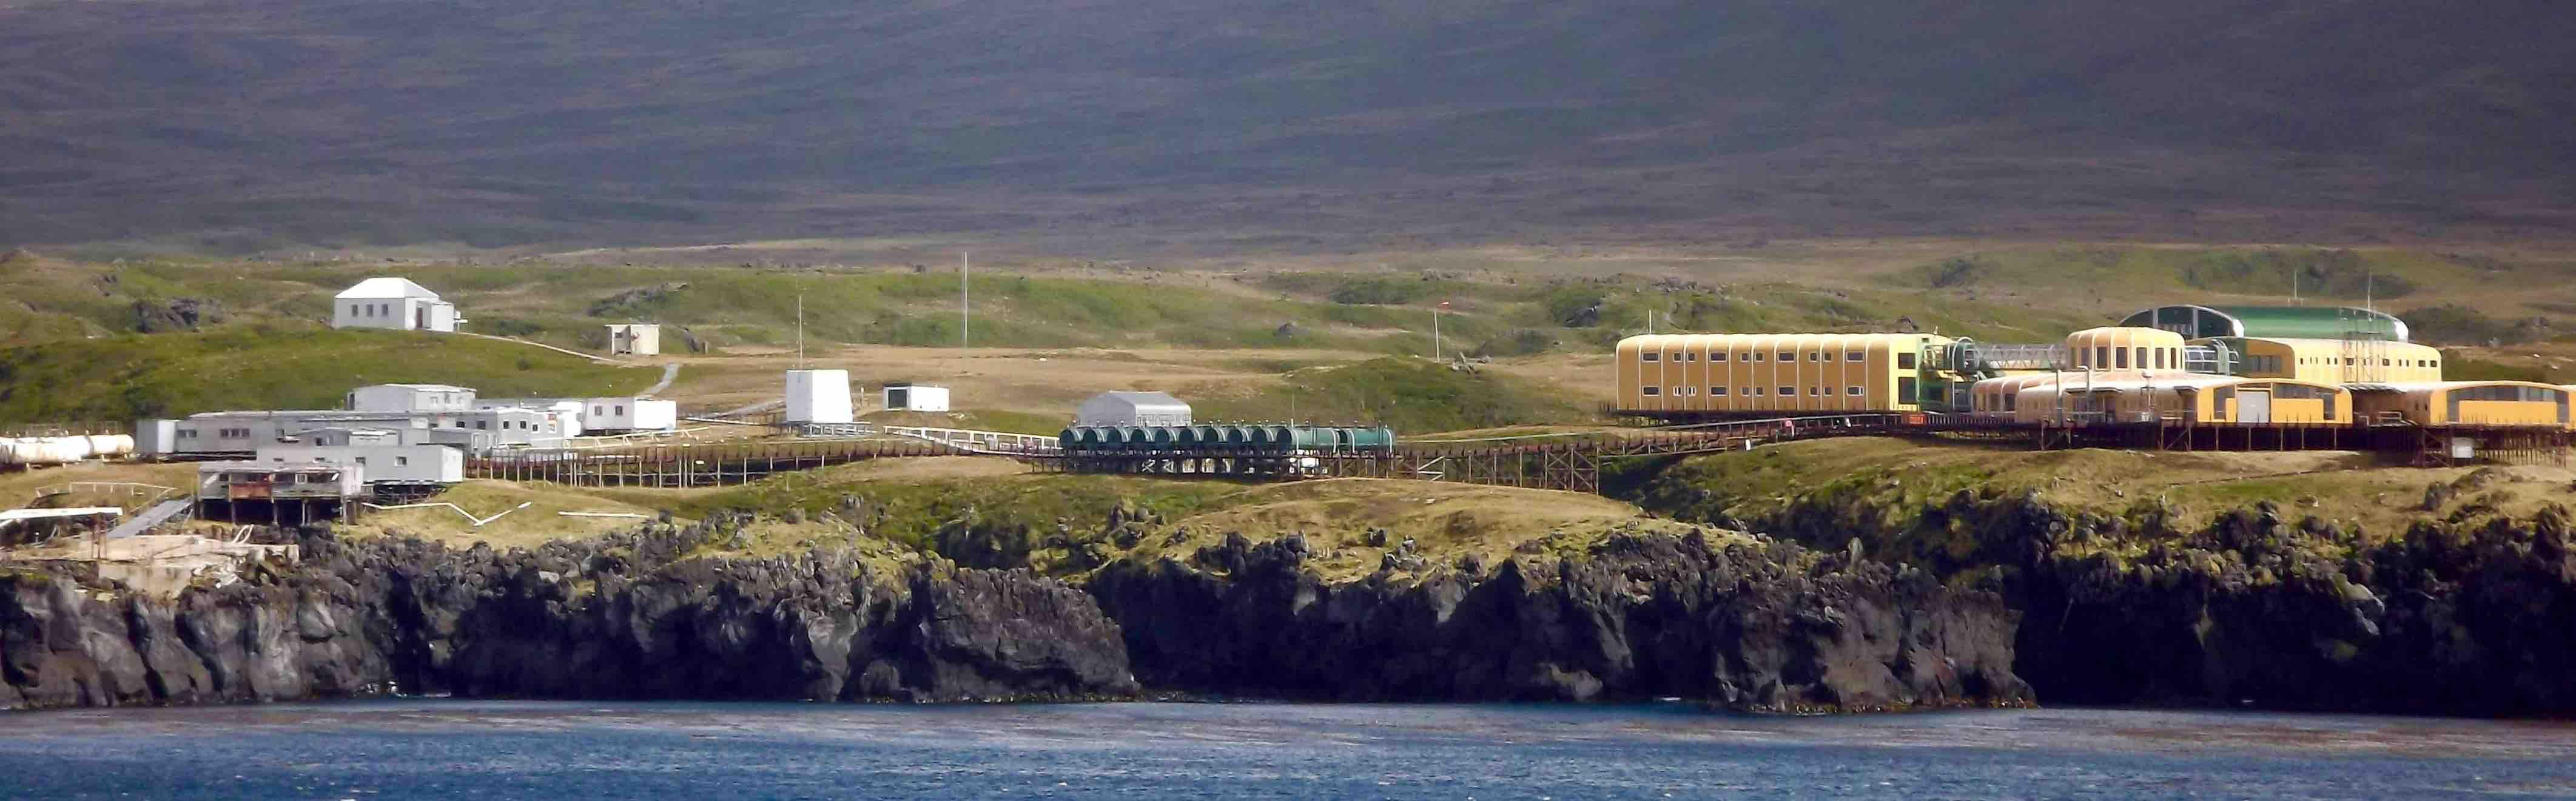
\includegraphics[width=\linewidth]{Figures/base}
	\caption{Marion Island new (yellow buildings) and old base (white buildings). The green building partially visible behind the new base is the emergency base that serves as a helipad and a hangar for helicopter operations.}
	\label{fig:base}
\end{figure}

The DEA owns the S. A. Agulhas II \footnote{\url{https://en.wikipedia.org/wiki/S. A. Agulhas II}}, a South African ice-breaking polar supply and research ship that services the island every year in April. During the relief voyage in April, three weeks are spent on the island deploying and maintaining \st{the existing} instruments. Marion Island \st{caters for various} \attention{has been traditionally used for the} research fields \attention{of space weather, geology,} \st{such as} meteorology, mammalogy, ornithology, and botany. The main Marion base accommodates all the researchers participating in the relief voyage and overwintering team members. Figure~\ref{fig:site} shows the nine rest huts (Kildalkey, Watertunnel, Cape Davis, Grey-headed, Mixed Pickle, Repettos, Rooks, Swartkops, and, Katedraal) that researchers use while traversing the island. The \prizm\ instrument was deployed at the \prizm\ site \attention{[``PRIZM site'' isn't very descriptive; replace this with e.g. 4km southwest of the main base]} (\ang{46;53;13}S, \ang{37;49;10.7}E) as the first radio astronomy experiment in Marion Island, followed by the \albatros\ \st{experiment} \attention{pathfinder instruments} on the same site. 

\begin{figure}
	\centering
	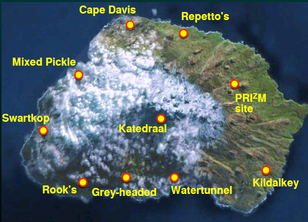
\includegraphics[width=\linewidth]{Figures/site}
	\caption{Marion Island rest huts and the \prizm\ site where the first radio astronomy instrument was deployed and subsequently \albatros\ pathfinder.}
	\label{fig:site}
\end{figure}

\section{Advantages of Observing from Marion Island}

\st{The discussion that follows is described by} \attention{This section presents a brief overview of the site selection process on Marion, and a full description is available in}~\citet{2019JAI.....850004P} \attention{[note the difference between citep, which places cites in parentheses, and citet, which includes cites as part of the text]}. In choosing the observing site for \prizm\ \attention{[don't forget to put the backslash at the end of prizm so that it doesn't gobble the following space; I've fixed here, but I'll leave it up to you to do a search and replace elsewhere]} and \albatros, several radio spectrum measurements were done on different sites, including the South African Karoo desert. The radio-quiet environment of Marion Island surpasses that of the South African Karoo desert, as shown in Figure~\ref{fig:karoo}. At Marion Island \st{site}, there is no evident detection of RFI contamination in the FM band\attention{, and the only significant RFI visible within the PRIZM operating range is} \st{besides the} Orbcomm satellite transmission \st{visible} at \SIrange{137}{138}{\mega\hertz} and the \SI{250}{\mega\hertz} FPGA clock artifact visible at \SI{125}{\mega\hertz}. The enhanced RFI from meteor scattering \attention{[expand and explain this a bit more: ionization trails scatter distant RFI sources]} is a common \st{threat} \attention{phenomenon} in several remote sites excluding Marion Island, as there have not been evident measurements of such RFI.

\begin{figure}
	\centering
	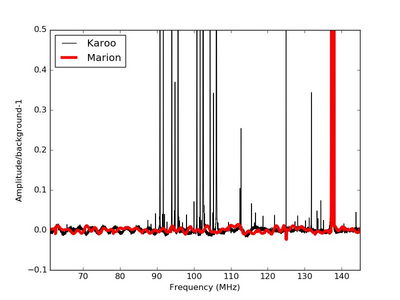
\includegraphics[width=\linewidth]{Figures/karoo}
	\caption{Comparison of radio spectrum on Marion (thick red) and in the Karoo desert (thin black). The fractional amplitude above a background fit to the raw and uncalibrated data without RFI excision. Orbcomm satellite transmission is visible at 137–138 MHz; there is no visible RFI in Marion's data. The feature at 125 MHz is an artifact of the 250 MHz FPGA clock and not due to RFI~\citep{2019JAI.....850004P}}
	\label{fig:karoo}
\end{figure}

Figure~\ref{fig:rfi} shows the RFI spectrum comparison between the \prizm deployment site \SI{4}{\kilo\metre} away from the island's main base. Locally generated RFI less impacts the \prizm site \attention{[rework this sentence to describe that we wanted a site for PRIZM that was far enough away from the main base to keep locally generated RFI at a minimum while still being a reasonable hiking distance]}. Junior's Kop situated between the deployment site and the island's main base provides enhanced RFI shielding of \SI{\sim60}{\decibel} \attention{[note that 60~dB is a combination of attenuation from the land mass in Junior's, plus the distance]}. The helicopter was operating near the base when the RFI measurements were taken and transmitting at a frequency of \SI{123.45}{\mega\hertz} \attention{[expand this sentence a bit more and explain that the helo transmission line was a fortuitous source of RFI that allowed us (roughly) calibrate the relative levels at Junior's vs the base]}.  \attention{Somewhere in here, you may also want to mention the constraint that we wanted a site with reasonably dry and even terrain, i.e. not in a mire. :-)}

\begin{figure}
	\centering
	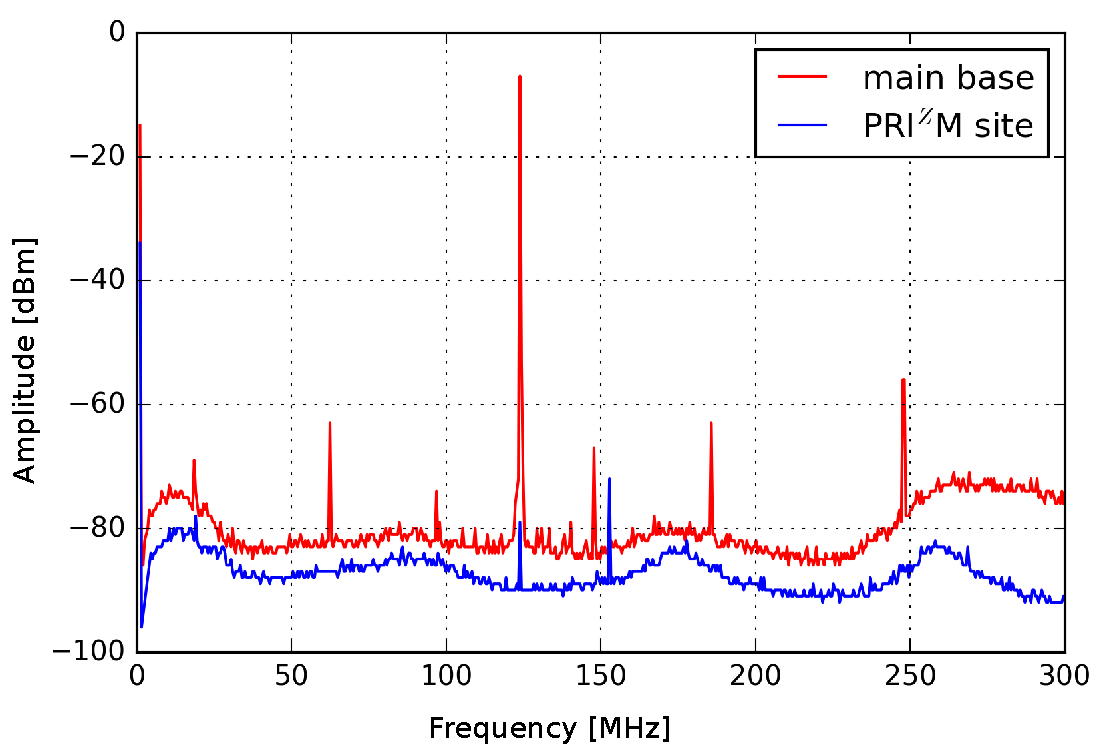
\includegraphics[width=\linewidth]{Figures/rfi}
	\caption{RFI measurement differentiated from the Marion base and the \prizm observing site. When the measurements were taken, the spectrum analyzer was set to max hold, and the measurement period coincided with the helicopter's operation near the base and transmitting at \SI{123.45}{\mega\hertz}. A rough benchmark of $\sim$60 dB signal suppression in received power at both locations arising from a combination of attenuation from Junior's kop and the distance between the \prizm site and the base. The peak at 156 MHz is a transmission from a handheld radio~\citep{2019JAI.....850004P}.}
	\label{fig:rfi}
\end{figure}

Figure~\ref{fig:IRI_model} shows the international reference ionosphere (IRI) model~\citep{ars-16-1-2018} predictions illustrating the minimum ionospheric plasma cutoff frequency during the last solar minima. The development of new low-frequency experiments is predominantly driven by the lack of knowledge of what lies in the sky at frequencies $\lessapprox$\SI{30}{\mega\hertz}.  According to the international reference ionospheric (IRI) model prediction, measurements of the sky at $\lessapprox$\SI{30}{\mega\hertz} do not look entirely impossible because, during the last solar \st{minima} \attention{minimum}, the ionospheric plasma cutoff frequency was \st{measured} \attention{predicted} to be $\sim$\SI{1.5}{\mega\hertz} at Marion Island. Since we are currently experiencing another solar minimum~\citep{2018NatCo...9.5209B}, it is an excellent opportunity to develop and implement new low-frequency observations. The prediction shows Marion Island, Dome C in Antarctica, and Hobart in Tasmania, where Reber performed his \SI{2}{\mega\hertz} observation. They have the potential to provide new views of the Earth's ionosphere, which absorbs and refracts at radio frequencies and becomes utterly opaque below the plasma cutoff frequency. \attention{[Since you've focused on the advantages of Marion, you may also want to include a couple of sentences about the drawbacks: limited access, Roaring 40s weather, mice, boundary conditions on equipment installs because it's an environmentally protected area, etc...but end on a positive note that although it's a somewhat steep price to pay, the reward is an unparalleled RF-quiet environment]} In the next two chapters, the \prizm\ and \albatros\ experiments are discussed in detail.

\begin{figure}
	\centering
	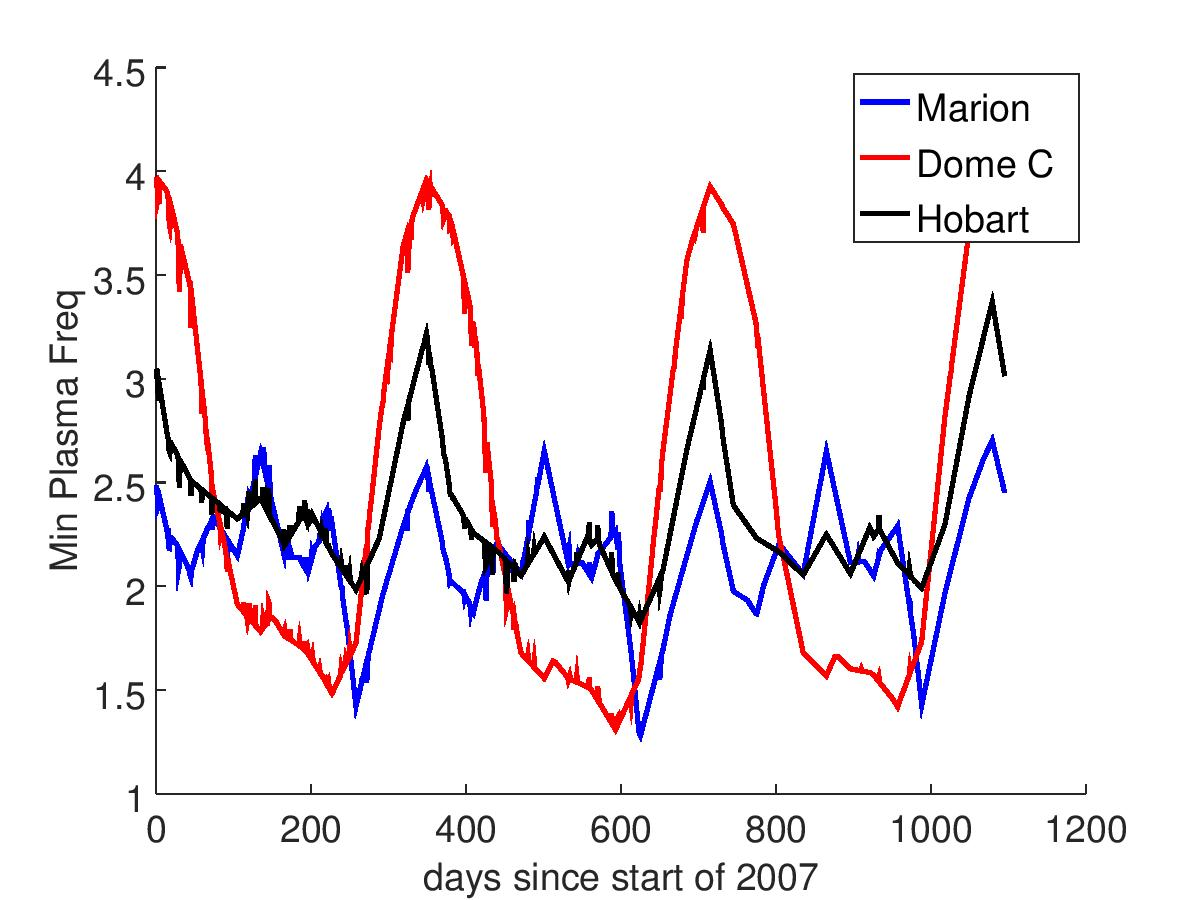
\includegraphics[width=\linewidth]{Figures/IRI_model}
	\caption{The International Reference Ionosphere model predictions illustrating the minimum ionospheric plasma cutoff frequency during last solar minima. At Marion Island, Dome C in Antarctica and Hobart in Tasmania the plasma frequency may drop as low as $\sim$\SI{1.5}{\mega\hertz}~\citep{2020arXiv200812208C}.}
	\label{fig:IRI_model}
\end{figure}
